%----------------------------------------------------------------------------------------
%	PACKAGES AND OTHER DOCUMENT CONFIGURATIONS
%----------------------------------------------------------------------------------------

\documentclass[12pt]{article}

\usepackage[margin=1in]{geometry}
\usepackage[brazil]{babel}
\usepackage[utf8]{inputenc}
\usepackage{textcomp}
\usepackage{float}
\usepackage{csquotes}
\usepackage[colorinlistoftodos]{todonotes}
\usepackage{caption}
\usepackage{commath}
\usepackage{subcaption}
\usepackage{hyperref}
\usepackage{amsmath}
\usepackage{amssymb}
\usepackage{indentfirst}
\usepackage{graphicx}
\usepackage{parskip}
\usepackage{setspace}
\usepackage{advdate}
\usepackage{url}
\usepackage[framed,numbered,autolinebreaks,useliterate]{mcode}
\usepackage[backend=biber, style=abnt-numeric, noslsn]{biblatex}
\usepackage{pdfpages}
\addbibresource{referencia.bib}

\DeclareCiteCommand{\supercite}[\mkbibsuperscript]
  {\iffieldundef{prenote}
     {}
     {\BibliographyWarning{Ignoring prenote argument}}%
   \iffieldundef{postnote}
     {}
     {\BibliographyWarning{Ignoring postnote argument}}}
  {\usebibmacro{citeindex}%
   \bibopenbracket\usebibmacro{cite}\bibclosebracket}
  {\supercitedelim}
  {}

\setlength{\parindent}{1cm}

\setlength{\marginparwidth}{2cm}
\begin{document}
\begin{titlepage}

\newcommand{\HRule}{\rule{\linewidth}{0.5mm}} 
\center
 
%----------------------------------------------------------------------------------------
%	HEADING SECTIONS
%----------------------------------------------------------------------------------------

\textsc{\LARGE Universidade de São Paulo}\\[1.5cm]
\textsc{\Large Escola Politécnica}\\[0.5cm] 
\textsc{\large MAP3121 - Métodos Numéricos e Aplicações (2020)}\\
\vspace{70mm}
%----------------------------------------------------------------------------------------
%	TITLE SECTION
%----------------------------------------------------------------------------------------

{\huge \bfseries Exercício Programa 2}\\[0.6cm]
\textsc{\large }\\[2.5cm]
 
%----------------------------------------------------------------------------------------
%	AUTHOR SECTION
%----------------------------------------------------------------------------------------
\vspace{60mm}
\begin{minipage}{0.4\textwidth}
\begin{flushleft} \large
\footnotesize{\textsc{Nomes}}\\
Elias Daleffi Rodrigues Rayes\\
Vinícius Marchioli\\


\end{flushleft}
\end{minipage}
~
\begin{minipage}{0.4\textwidth}
\begin{flushright} \large
\footnotesize{\textsc{NUSP}}\\
10823848\\
10774232\\

\end{flushright}
\end{minipage}\\[7.5cm]


%----------------------------------------------------------------------------------------
%	LOGO SECTION
%----------------------------------------------------------------------------------------


\vfill 

\end{titlepage}
%------------------- Table of contents --------------------%
\tableofcontents 
\clearpage
%------------------- Comeco do texto ----------------------%
\begin{spacing}{1.5}

\section{Tarefa A}

Na primeira tarefa, a partir do desenvolvido no Exercício Programa 1, será empregado o método de Crank-Nicolson, cujo termo geral é descrito pela relação mostrada em \eqref{crankNicolson}, para resolução numérica da equação diferencial de calor dada por \eqref{calor1}, \eqref{calor2}, \eqref{calor3} e \eqref{calor4} com condição inicial e de fronteira nulas $\left(u_0(x) = g_1(t) = g_2(t) = 0 \right)$.

\begin{equation} \label{crankNicolson}
u_{i}^{k+1} = u_i^k + \dfrac{\lambda}{2}((u^{k+1}_{i-1} - 2u^{k+1}_{i} + u_{i+1}^{k+1}) + (u^{k}_{i-1} -2u^{k}_i + u^k_{i+1})) + \dfrac{\Delta t}{2}(f(x_i,t_k) + f(x_{i},t_{k+1}))
\end{equation}

\begin{gather}
u_{t}(t,x) = u_{x x}(t,x) + f(t,x) \;\; \text{em} \;\; [0,T]\times[0,1] \label{calor1}\\
u(0,x)=u_0(x) \;\;\text{em}\;\; [0,1] \label{calor2}\\
u(t,0)=g_1(t) \;\;\text{em}\;\; [0,T] \label{calor3}\\
u(t,1)=g_2(t) \;\;\text{em}\;\; [0,T] \label{calor4}
\end{gather}


Dado um conjunto de pontos $p_1, p_2, \cdots, p_{n f}$, deve-se gerar os vetores $u_k(T,x_i),\;i = 1, 2, \cdots, N - 1 $ que se referem às distribuições de temperatura na barra, no instante $T$ ($t=1$), a partir da ação de cada fonte de calor pontual da forma $f(t,x)=r(t)g_h^k(x),\; k = 1, 2, \cdots, nf$, sendo $r(t) = 10\cdot(1+\cos(5t))$, com $g_h^k(x)$ e $f(t,x)$ nas formas \eqref{regiao_pontual} e \eqref{fonte_pontual}. 

\begin{equation}\label{regiao_pontual}
g_{h}^k(x) =\begin{cases}
    \dfrac{1}{h},\;\; \text{se} \;\; p-\dfrac{h}{2} \leq x \leq p + \dfrac{h}{2} \\
    0,\;\; \text{caso contrário.}
\end{cases}
\end{equation}

\begin{equation}\label{fonte_pontual}
f(t,x) =\begin{cases}
     \dfrac{10\cdot(1 + \cos(5t))}{\Delta x},\;\; \text{se} \;\; p-\dfrac{\Delta x}{2} \leq x \leq p + \dfrac{\Delta x}{2} \\
    0,\;\; \text{caso contrário.}
\end{cases}
\end{equation}

\clearpage
É relevante ressaltar que, no escopo deste exercício, obter todas as distribuições de temperatura  $u_k(T,x_i)$ individualmente, resultantes da ação de uma única fonte, corresponde a encontrar um conjunto de vetores linearmente independentes entre si que compõem uma base, cuja dimensão é o número total de fontes pontuais. O agregado de tais fontes corresponde à uma forçante da forma $f(t,x) = r(t)\sum_{k=1}^{n f}{a_kg^k_h(x)}$. Os coeficientes $a_k$ representam as contribuições de cada fonte para a temperatura final e serão determinados ao fim do exercício programa.

Em relação ao que já foi implementado no exercício programa 1, foi necessário, simplesmente, ajustar a função $f(t,x)$ do método de Crank-Nicolson às condições do enunciado (considerar $r(t) = 10\cdot(1+\cos(5t))$) e encontrar a distribuição final de calor para cada $p$.
Assim, para a solução desse passo, foi utilizada a decomposição $A=LDL^{t}$ para uma matriz A esparsa, tridiagonal e positivamente definida e, a partir disso, pode-se calcular, de modo mais eficiente, a solução para o sistema linear que descreve o termo geral \eqref{crankNicolson} para cada instante de tempo. Ao se fazer esse procedimento para cada fonte e extrair das soluções o instante final, encontra-se a base desejada, sobre qual deve-se projetar $u_T(x)$. 

\section{Tarefa B}

Quando conhecida a distribuição de temperatura $u_T = r(t)\sum_{k=1}^{n f}{a_k u_k(T, x)}$, no instante $T$, é de interesse determinar os coeficientes $a_k$ que minimizam a expressão \eqref{rms}. Dessa forma, deve-se resolver um problema de melhor aproximação, ou seja, de mínimos quadrados. É importante ressaltar que os extremos do intervalo têm seus valores conhecidos pelas condições de contorno impostas e, por isso, não necessitam ser contemplados pela expressão \eqref{rms}.

\begin{equation}\label{rms}
E_2 = \sqrt{\Delta x \sum_{i=1}^{N - 1} \left(u_T(x_i) - \sum_{k=1}^{n f}{a_k u_k(T,x_i)}\right)^2}  
\end{equation}

Em posse dos vetores que compõem a base, para a solução do problema de minimização de distâncias e obtenção dos coeficientes (intensidade de cada fonte), deve-se montar e resolver o sistema representado em \eqref{matrix:sitema_normal}. Para tal, é necessário implementar a rotina que calcula o produto interno, mostrado em \eqref{prod_int}.

\begin{equation}\label{matrix:sitema_normal}
    \renewcommand*{\arraystretch}{0.75}
    \begin{bmatrix}
        \langle u_1, u_1\rangle & \langle u_2, u_1\rangle & \cdots & \langle u_{n f}, u_1\rangle\\
        \langle u_1, u_2\rangle & \langle u_2, u_2\rangle & \cdots & \langle u_{n f}, u_2\rangle\\
        \vdots  & \vdots & \ddots & \vdots \\
        \langle u_1, u_{n f}\rangle & \langle u_2, u_{n f}\rangle & \cdots & \langle u_{n f},  u_{n f}\rangle
    \end{bmatrix}
    \begin{bmatrix}
    a_1 \\
    a_2 \\
    \vdots \\
    a_{n f}
    \end{bmatrix}
    =
    \begin{bmatrix}
    \langle u_T, u_1\rangle \\
    \langle u_T, u_2\rangle \\
    \vdots \\
    \langle u_T, u_{n f}\rangle
    \end{bmatrix}
\end{equation}

\begin{equation}\label{prod_int}
\langle u, v\rangle = \sum_{i=1}^{N - 1}{u(x_i) v(x_i)}
\end{equation}


\section{Tarefa C}

Ao contrário do exercício programa 1, cujo sistema a ser resolvido era constituído por uma matriz tridiagonal simétrica, as matrizes que compõem o sistema \eqref{matrix:sitema_normal}, não são esparsas. Por conseguinte, para a otimização do tempo e dos recursos computacionais empregados, é feita decomposição\supercite{burden&faires} $LDL^t$ sendo $L$ uma matriz triangular inferior e $D$ uma matriz diagonal, como visto em \eqref{matrix:ldlt}.


\begin{align}\label{matrix:ldlt}
    L =
    \renewcommand*{\arraystretch}{0.75}
    \begin{bmatrix}
    1 &&&&&\\
    l_{2,1}&\ddots &&&&\\
    &\ddots &1&&&\\
    \vdots &\dots &l_{j+1,j}&1&&\\
    &&\vdots &\ddots &\ddots &\\
    l_{N,1}&\dots &l_{N,j}&\dots &l_{N,N-1}&1
    \end{bmatrix} &&
    D =
    \renewcommand*{\arraystretch}{0.8}
    \begin{bmatrix}
    d_1 &0&&\dots&&0\\
    0& d_2 &&&&\\
    & &\ddots&&&\vdots\\
    \vdots& & & d_j &&\\
    &&&& \ddots&0\\
    0&&\dots&&0& d_{N}
    \end{bmatrix} &&
\end{align}


\begin{gather}
    D_{j}=A_{jj}-\sum _{k=1}^{j-1}L_{jk}^{2}D_{k}, \\
    L_{ij}={\frac {1}{D_{j}}}\left(A_{ij}-\sum _{k=1}^{j-1}L_{ik}L_{jk}D_{k}\right)\quad {\text{para }}i>j.
\end{gather}

A solução da equação matricial pode ser feita em três partes, resolvendo sistemas lineares triangulares simples em cada passo. Podemos, então, decompor $A = LDL^t$ em:

\setlength{\abovedisplayskip}{0.05cm}
\setlength{\belowdisplayskip}{0.2cm}
\begin{gather*}
    L z = b \\
	D y = z \\
	L^t x = y 
\end{gather*}

\section{Testes}

Após a implementação das rotinas descritas nas tarefas, foram executados quatro diferentes testes para a comprovação do correto funcionamento do programa. A persistência das saída de cada teste foi feita através de arquivos \textit{.txt} cujos nomes seguem a convenção $\text{Output } + <\text{letra do teste}> + <\text{valor de N}>$. Por exemplo, o arquivo nomeado \textit{OutputC2048.txt} refere-se ao teste C, com $N=2048$. Em todos os testes, foi considerado $r(t)=10\cdot(1+\cos(5t))$ e $T=1$.

O \textit{script} de MATLAB utilizado para gerar as curvas encontra-se no Apêndice \ref{cod_MATLAB}.

%----------------------------------------------------------------------------------------%
\subsection{Teste A}

Primeiramente, considerou-se uma única fonte pontual ($n f =1$), $N=128$, $p=0,35$ e definiu-se $u_T(x_i) = 7\cdot u_1(x_i)$, de modo que $u_1(x_i)$ é a solução do método de Crank-Nicolson para uma única fonte pontual, localizada em $p$.

Como, de antemão, conhece-se a contribuição da única fonte pontual existente ($a_1=7$), essa tarefa tem como objetivo comprovar o funcionamento adequado do código desenvolvido. Após a resolução de um sistema trivial $1\times 1$, obteve-se o resultado esperado $a_1=7$. A figura \ref{fig:testeA} mostra que a curva conhecida $u_T$ e a curva reconstruída $7\cdot u_1$ são, de fato, iguais. O erro obtido ($1,142742\cdot10^{-15}$), pela equação \eqref{rms}, deve-se apenas à aproximações numéricas na resolução do sistema.

\begin{figure}[H]
    \centering
    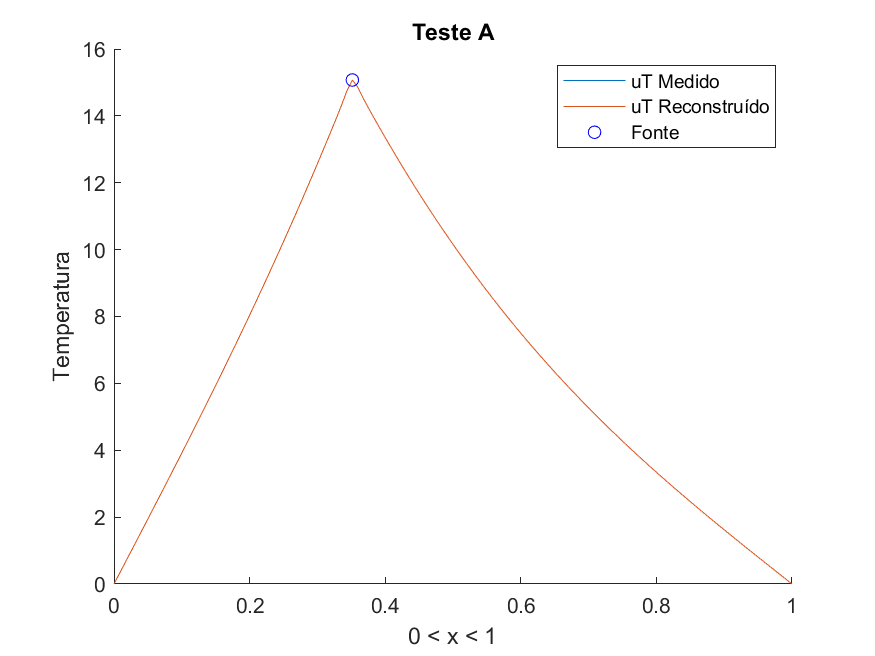
\includegraphics[width=0.75\linewidth]{Imagens/FigA128.png}
    \caption{Distribuição de temperatura do teste A, com destaque na fonte pontual}
    \label{fig:testeA}
\end{figure}

%----------------------------------------------------------------------------------------%
\subsection{Teste B}

No teste B, ainda com $N=128$, há um aumento no número de fontes. Agora, têm-se $n f = 4$ com $p_1 = 0,15$, $p_2 = 0,3$, $p_3 = 0,7$ e $p_4 = 0,8$. Novamente, é definido $u_T(x_i) = 2,3\cdot u_1(T, x_i) + 3,7\cdot u_2(T, x_i) + 0,3\cdot u_3(T, x_i) + 4,2\cdot u_4(T, x_i)$, de modo que a solução $a=[a_1,a_2,a_3,a_4]$ já é conhecida.

Nesse caso, almeja-se testar e comprovar o funcionamento da rotina de decomposição $LDL^t$ e resolução de sistemas maiores, como o mostrado em \eqref{matrix:4x4}. O erro $E_2$ obtido foi de $3,780624\cdot10^{-15}$ e deve-se, simplesmente, a arredondamentos sucessivos. A figura \ref{fig:testeB} mostra as curvas obtidas.

\begin{equation}\label{matrix:4x4}
    \renewcommand*{\arraystretch}{0.75}
    \begin{bmatrix}
        \langle u_1, u_1\rangle & \langle u_2, u_1\rangle & \langle u_3, u_1\rangle & \langle u_4, u_1\rangle\\
        \langle u_1, u_2\rangle & \langle u_2, u_2\rangle & \langle u_3, u_2\rangle & \langle u_4, u_2\rangle\\
        \langle u_1, u_3\rangle & \langle u_2, u_3\rangle & \langle u_3, u_3\rangle & \langle u_4, u_3\rangle\\
        \langle u_1, u_4\rangle & \langle u_2, u_4\rangle & \langle u_3, u_4\rangle & \langle u_4,  u_4\rangle
    \end{bmatrix}
    \begin{bmatrix}
    a_1 \\
    a_2 \\
    a_3 \\
    a_4
    \end{bmatrix}
    =
    \begin{bmatrix}
    \langle u_T, u_1\rangle \\
    \langle u_T, u_2\rangle \\
    \langle u_T, u_3\rangle \\
    \langle u_T, u_4\rangle
    \end{bmatrix}
\end{equation}


\begin{figure}[H]
    \centering
    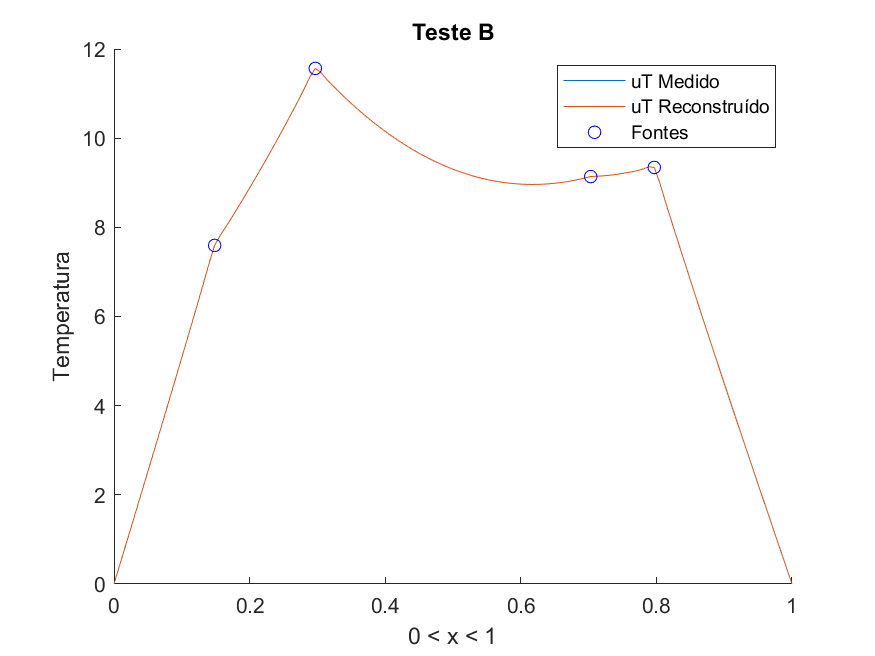
\includegraphics[width=0.75\linewidth]{Imagens/FigB128.png}
    \caption{Distribuição de temperatura do teste B}
    \label{fig:testeB}
\end{figure}

%----------------------------------------------------------------------------------------%
\subsection{Teste C}

A partir de um arquivo (\textit{teste.txt}), que fornece a posição de $n f=10$ fontes pontuais e a distribuição de temperatura $u_T(x_i)$ em $T=1$, deve-se encontrar os coeficientes $a_k$ que correspondem às intensidades de cada fonte, construindo a solução que resolve o problema inverso.

O arquivo fornece dados para uma malha de discretização $\Delta x = \dfrac{1}{2048}$ e, para os casos em que $N < 2048$, pontos igualmente espaçados são armazenados, desde que $N$ escolhido pelo usuário seja um submúltiplo de 2048.

As figuras \ref{fig:testeC_128}, \ref{fig:testeC_256}, \ref{fig:testeC_512}, \ref{fig:testeC_1024} e \ref{fig:testeC_2048} mostram as curvas geradas para os casos em que $N = 128,\;256,\;512,\;1024\;\text{e}\;2048$, respectivamente. Não é possível, a partir de $N=256$, notar diferenças visuais significativas entre as curvas.

Os erros $E_2$ obtidos pela equação \eqref{rms} variam entre $2,445340\cdot10^{-2}$ e $3,591445\cdot10^{-12}$ e podem ser vistos na tabela \ref{table:errosC} e na figura \ref{fig:Erro_TesteC}.

\begin{table}
	\begin{minipage}{0.65\linewidth}
        \centering
        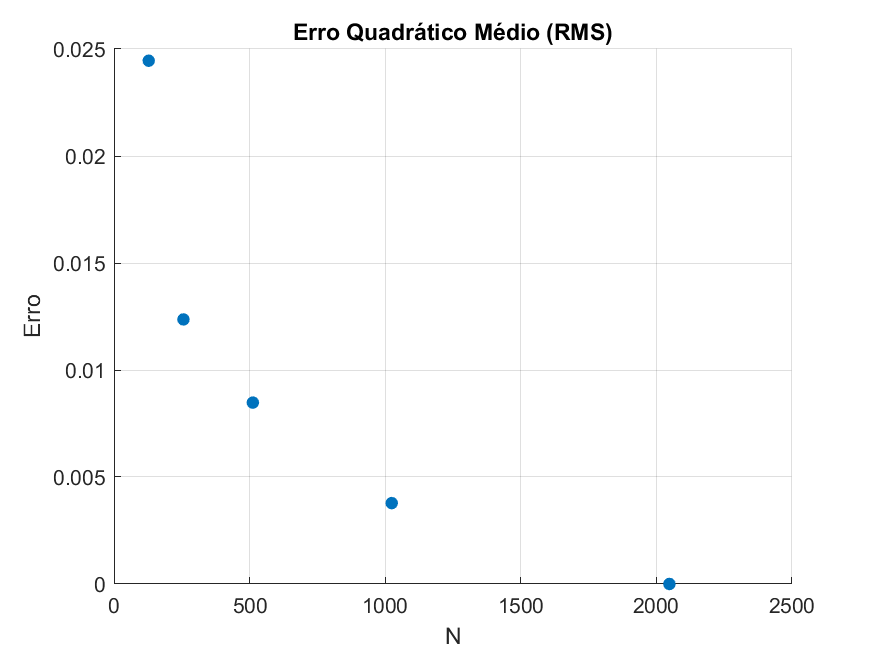
\includegraphics[width=1\linewidth]{Imagens/ErrosC.png}
        \captionof{figure}{Erros do teste C}
        \label{fig:Erro_TesteC}
	\end{minipage}
	\begin{minipage}{0.32\linewidth}
        \centering 
        \begin{tabular}{c c} 
        \hline\hline 
        \rule{0pt}{3ex} 
        N & Erro máximo\\ [0.5ex] 
        \hline 
        \rule{0pt}{4ex}
                128  & $2,445340   \cdot 10^{-2}$  \\ 
                256  & $1,236346  \cdot 10^{-2}$   \\ 
                512  & $8,476628 \cdot 10^{-3}$  \\ 
                1024 & $3,779310  \cdot 10^{-3}$ \\ 
                2048 & $3,591445  \cdot 10^{-12}$ \\ 
        \hline
        \end{tabular}
        \caption{Erros do teste C} 
        \label{table:errosC}
	\end{minipage}
	\hfill
\end{table}
\vspace{0.1cm}

Os coeficientes $a_k$ podem ser visualizados na tabela \ref{tabelaCoefc}. Vê-se convergência dos coeficientes conforme refina-se a malha, com o aumento de $N$, uma vez que os valores de erro (figura \ref{fig:Erro_TesteC} e tabela \ref{table:errosC}) decrescem consideravelmente.

\vspace{0.5cm}
\begin{table}[H]
\centering
\begin{tabular}{c c c c c c} 
\hline\hline 
\rule{0pt}{3ex} 
Posição da fonte & $N=128$ & $N=256$ & $N=512$ & $N=1024$ & $N=2048$\\ [0.5ex] 
\hline 
\rule{0pt}{4ex}
        0.15 & 1.209123 & 0.904501 & 0.928688 & 1.007281 & 1.0 \\ 
        0.20 & 4.839259 & 5.077573 & 5.053708 & 4.992443 & 5.0 \\ 
        0.30 & 1.887241 & 2.100854 & 2.043701 & 1.985877 & 2.0 \\ 
        0.35 & 1.583400 & 1.414156 & 1.467671 & 1.513258 & 1.5 \\
        0.50 & 2.214504 & 2.229245 & 2.196763 & 2.192693 & 2.2 \\ 
        0.60 & 3.121295 & 3.104614 & 3.091131 & 3.095153 & 3.1 \\
        0.70 & 0.377340 & 0.509453 & 0.637588 & 0.652327 & 0.6 \\
        0.73 & 1.492348 & 1.386509 & 1.271687 & 1.253790 & 1.3 \\
        0.85 & 3.975139 & 3.949879 & 3.878095 & 3.879667 & 3.9 \\
        0.90 & 0.404145 & 0.414893 & 0.530557 & 0.529737 & 0.5 \\
        [1ex]
\hline
\end{tabular}
    \caption{Coeficientes obtidos para o teste C}
    \label{tabelaCoefc}
\end{table}

\clearpage
\begin{figure}[ht!]
\centering
\caption{Distribuição de temperatura do teste C}
\captionsetup[subfigure]{justification=centering}
    \begin{subfigure}[t]{.485\linewidth}
        \centering
        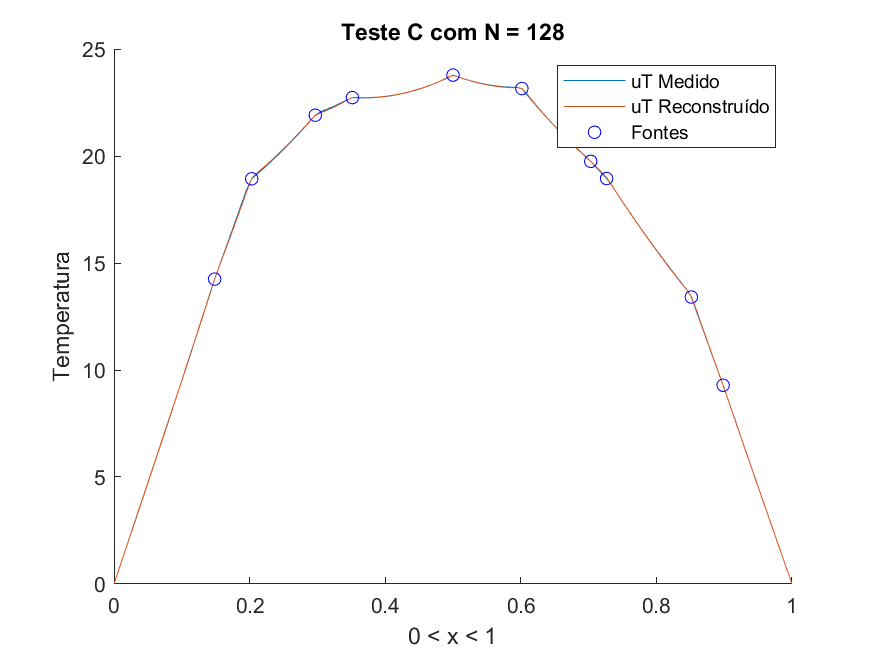
\includegraphics[width=1\linewidth]{Imagens/FigC128.png}
        \caption{$N=128$}
        \label{fig:testeC_128}
    \end{subfigure}
    \begin{subfigure}[t]{.485\linewidth}
        \centering
        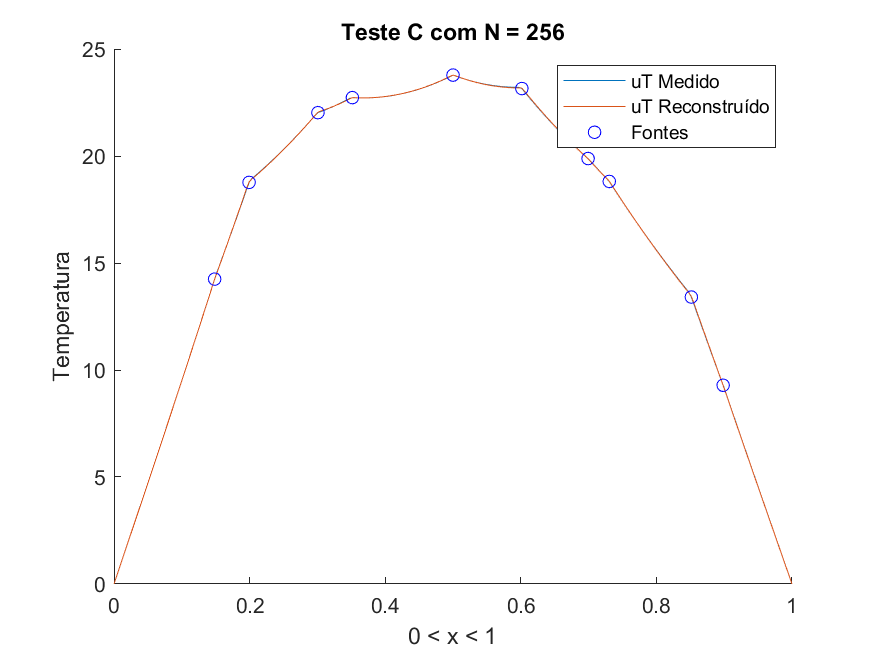
\includegraphics[width=1\linewidth]{Imagens/FigC256.png}
        \caption{$N=256$}
        \label{fig:testeC_256}
    \end{subfigure}
    \begin{subfigure}[t]{.485\linewidth}
        \centering
        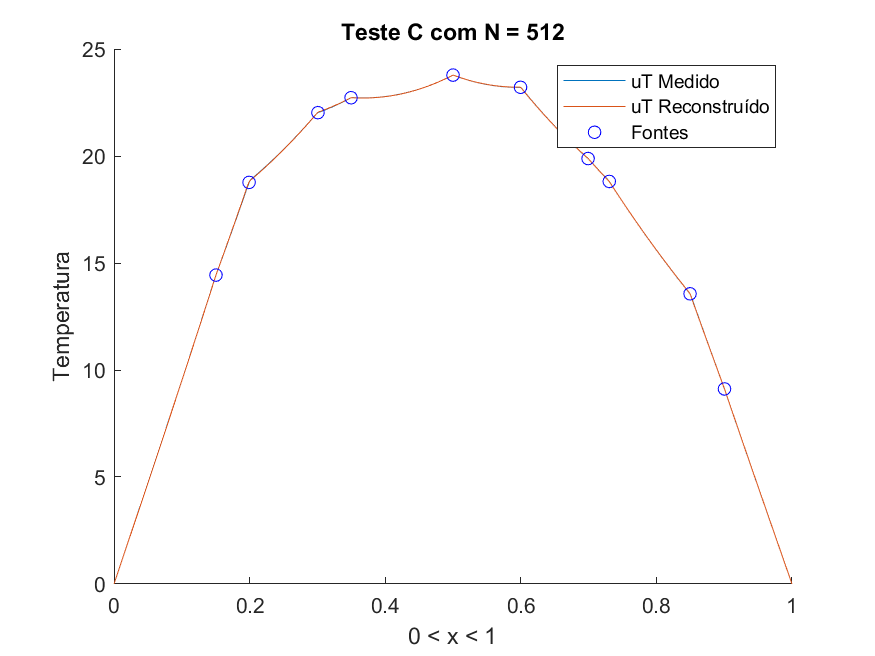
\includegraphics[width=1\linewidth]{Imagens/FigC512.png}
        \caption{$N=512$}
        \label{fig:testeC_512}
    \end{subfigure}
    \begin{subfigure}[t]{.485\linewidth}
        \centering
        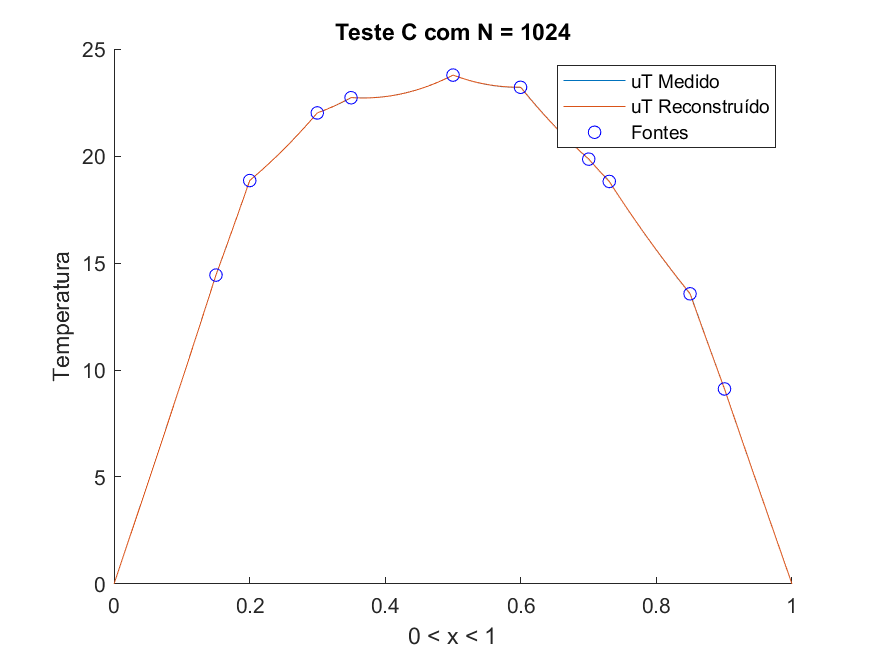
\includegraphics[width=1\linewidth]{Imagens/FigC1024.png}
        \caption{$N=1024$}
        \label{fig:testeC_1024}
    \end{subfigure}
    \begin{subfigure}[t]{.485\linewidth}
        \centering
        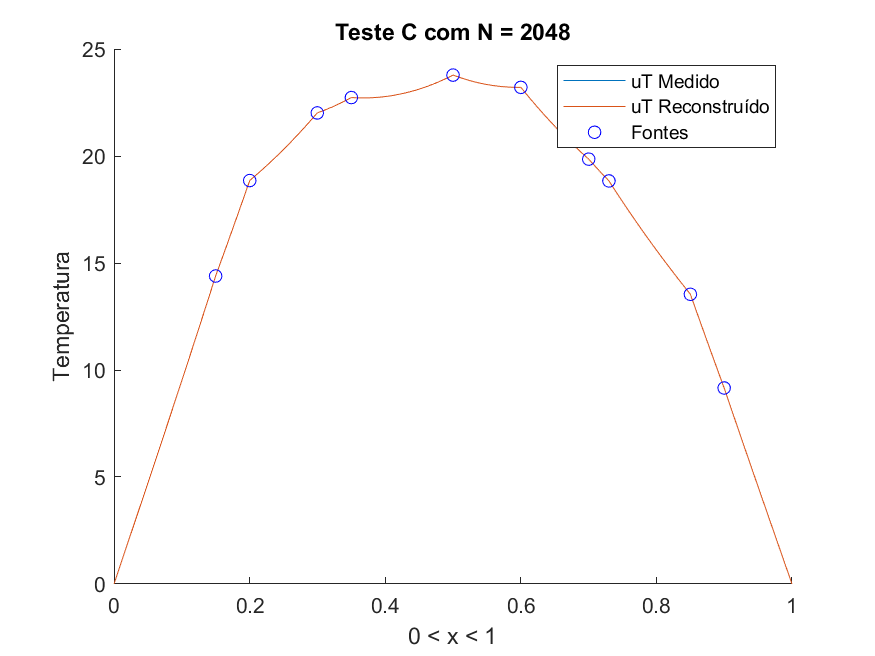
\includegraphics[width=1\linewidth]{Imagens/FigC2048.png}
        \caption{$N=2048$}
        \label{fig:testeC_2048}
    \end{subfigure}
\end{figure}
%----------------------------------------------------------------------------------------%
\subsection{Teste D}

Por último, a partir do mesmo arquivo \textit{.txt} do teste anterior, acrescentou-se ruído à distribuição de temperatura já conhecida. Tal ruído segue a forma $1 +\;r \epsilon$, sendo proporcional à curva original, com $\epsilon = 0,01$ e $r$ um número aleatório entre $-1$ e $1$, sendo que cada posição do vetor $u_T(x_i)$ é multiplicada por um destes valores gerados aleatoriamente.

No programa, feito em C++14, foi utilizado um PRNG, ou gerador de números pseudo-randômicos, como fonte do valor de $r$. Nesse caso, foi escolhido um Mersenne Twister, que é disponível livremente na linguagem\supercite{cpprandom} e é utilizado largamente na computação. Tal implementação requer uma semente, e para isso, utilizou-se um relógio de alta resolução\supercite{clock}, isto é, o tempo é a fonte de entropia. Assim, a partir desses dispositivos, é possível atingir uma distribuição numérica uniforme que, embora não seja realmente aleatória, é inteiramente adequada para os objetivos em questão.

As figuras \ref{fig:testeD_128}, \ref{fig:testeD_256}, \ref{fig:testeD_512}, \ref{fig:testeD_1024} e \ref{fig:testeD_2048} mostram as curvas geradas para os casos em que $N = 128,\;256,\;512,\;1024\;\text{e}\;2048$, respectivamente. Pela forma em que os fatores aleatórios são incorporados ao vetor, é possível notar um maior nível de ruído para maiores valores de temperatura.

Os erros $E_2$ obtidos pela equação \eqref{rms} permanecem em torno de $0,1$ e podem ser vistos individualmente, bem como os coeficientes $a_k$ obtidos, na saída do programa. É possível explicar tal comportamento para o erro devido ao ruído introduzido na distribuição. Sabendo-se que o valor de $1 +\;r \epsilon$ varia uniformemente, de forma aleatória, entre 99\% e 101\% de $u_T(x_i)$, pode-se estimar o valor do erro quadrático médio, ou seja, a medida do segundo momento\supercite{moment} do erro entre a curva de regressão e $u_T$ medido (ruidoso), deve ser em torno de 1\%. Portanto, o valor RMS do EQM, ou sua raiz quadrada, como descrito em \eqref{rms}, deve valer 0,1.

\begin{figure}[H]
\centering
\caption{Distribuição de temperatura do teste D}
\captionsetup[subfigure]{justification=centering}
    \begin{subfigure}[t]{.485\linewidth}
        \centering
        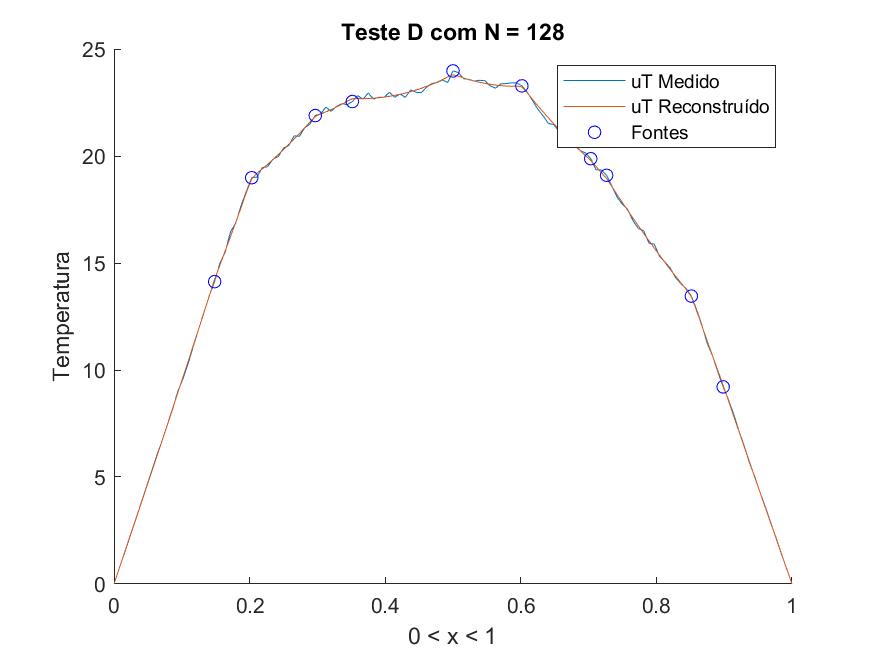
\includegraphics[width=1\linewidth]{Imagens/FigD128.png}
        \caption{$N=128$}
        \label{fig:testeD_128}
    \end{subfigure}
    \begin{subfigure}[t]{.485\linewidth}
        \centering
        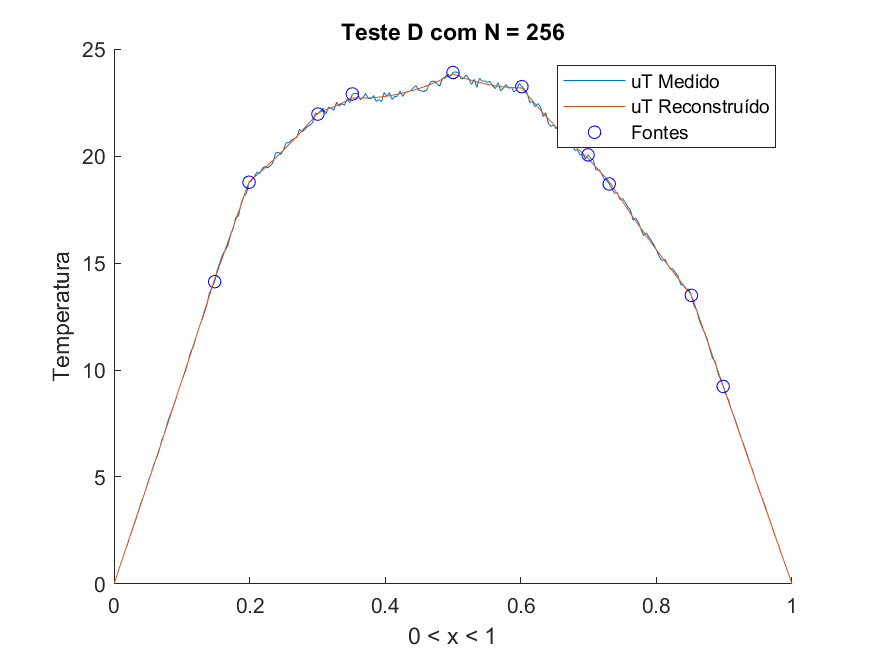
\includegraphics[width=1\linewidth]{Imagens/FigD256.png}
        \caption{$N=256$}
        \label{fig:testeD_256}
    \end{subfigure}
    \begin{subfigure}[t]{.485\linewidth}
        \centering
        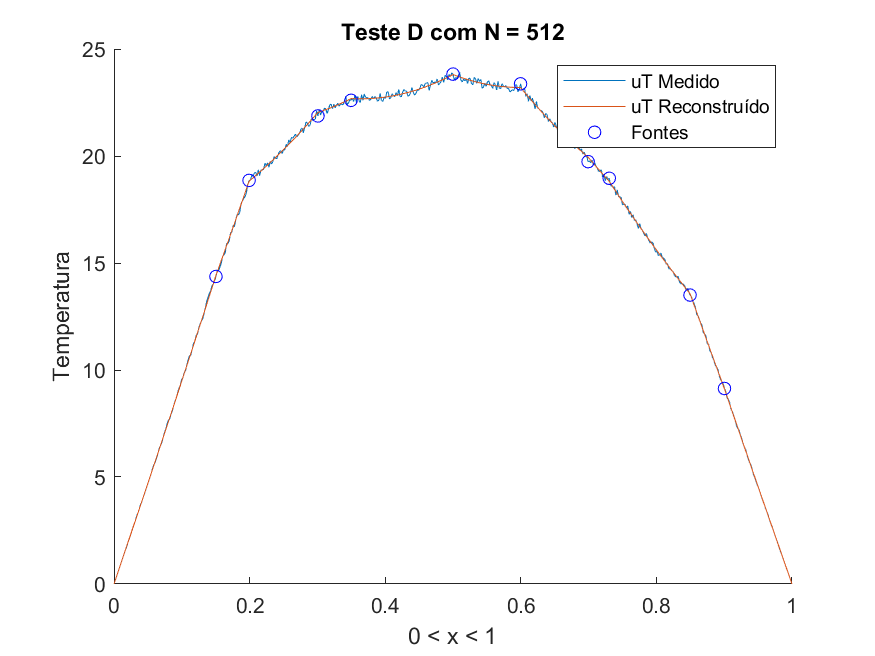
\includegraphics[width=1\linewidth]{Imagens/FigD512.png}
        \caption{$N=512$}
        \label{fig:testeD_512}
    \end{subfigure}
    \begin{subfigure}[t]{.485\linewidth}
        \centering
        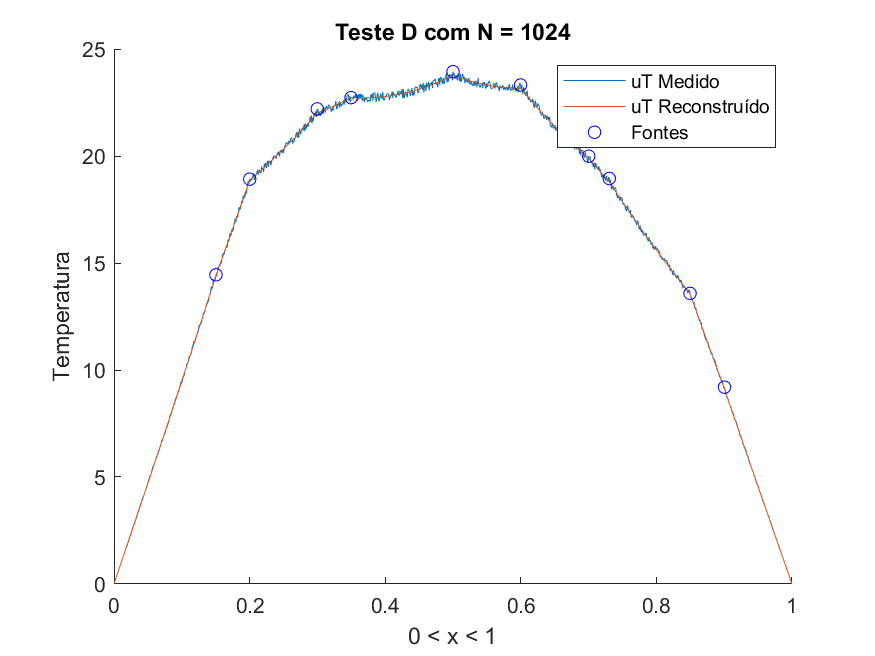
\includegraphics[width=1\linewidth]{Imagens/FigD1024.png}
        \caption{$N=1024$}
        \label{fig:testeD_1024}
    \end{subfigure}
    \begin{subfigure}[t]{.485\linewidth}
        \centering
        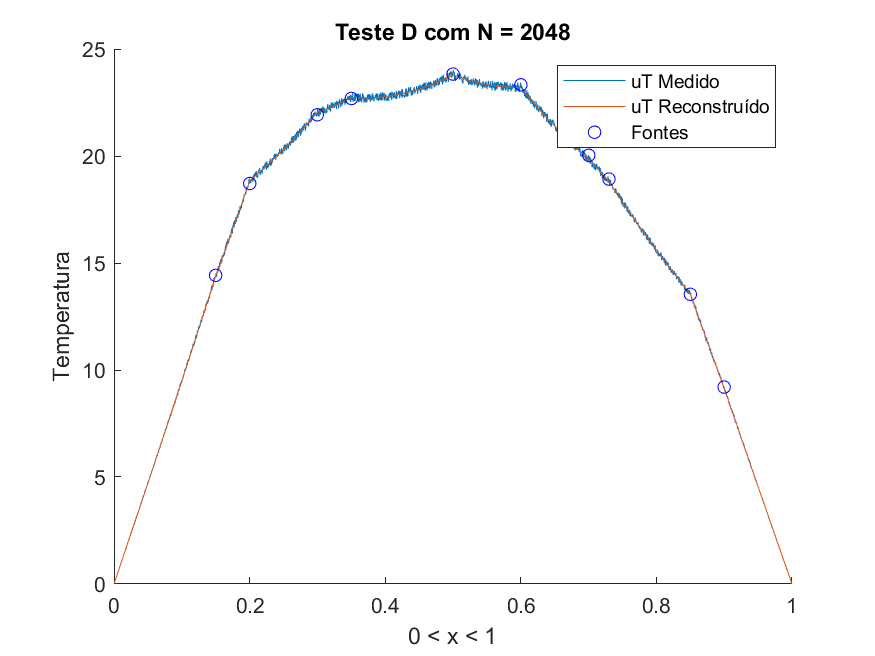
\includegraphics[width=1\linewidth]{Imagens/FigD2048.png}
        \caption{$N=2048$}
        \label{fig:testeD_2048}
    \end{subfigure}
\end{figure}

%----------------------------------------------------------------------------------------%
%------------------- Referências --------------------%  
\clearpage
\addcontentsline{toc}{section}{Referências}
\nocite{*}
\printbibliography

\newpage
\appendix
\section*{Apêndices}
\addcontentsline{toc}{section}{Apêndices}
\renewcommand{\thesubsection}{\Alph{subsection}}

%------------------- MATLAB --------------------%

\subsection{Código em MATLAB para gerar as curvas}\label{cod_MATLAB}

\lstinputlisting{EP2Testes.m}
\newpage

\subsection{LEIAME}
\begin{figure}[H]
    \centering
    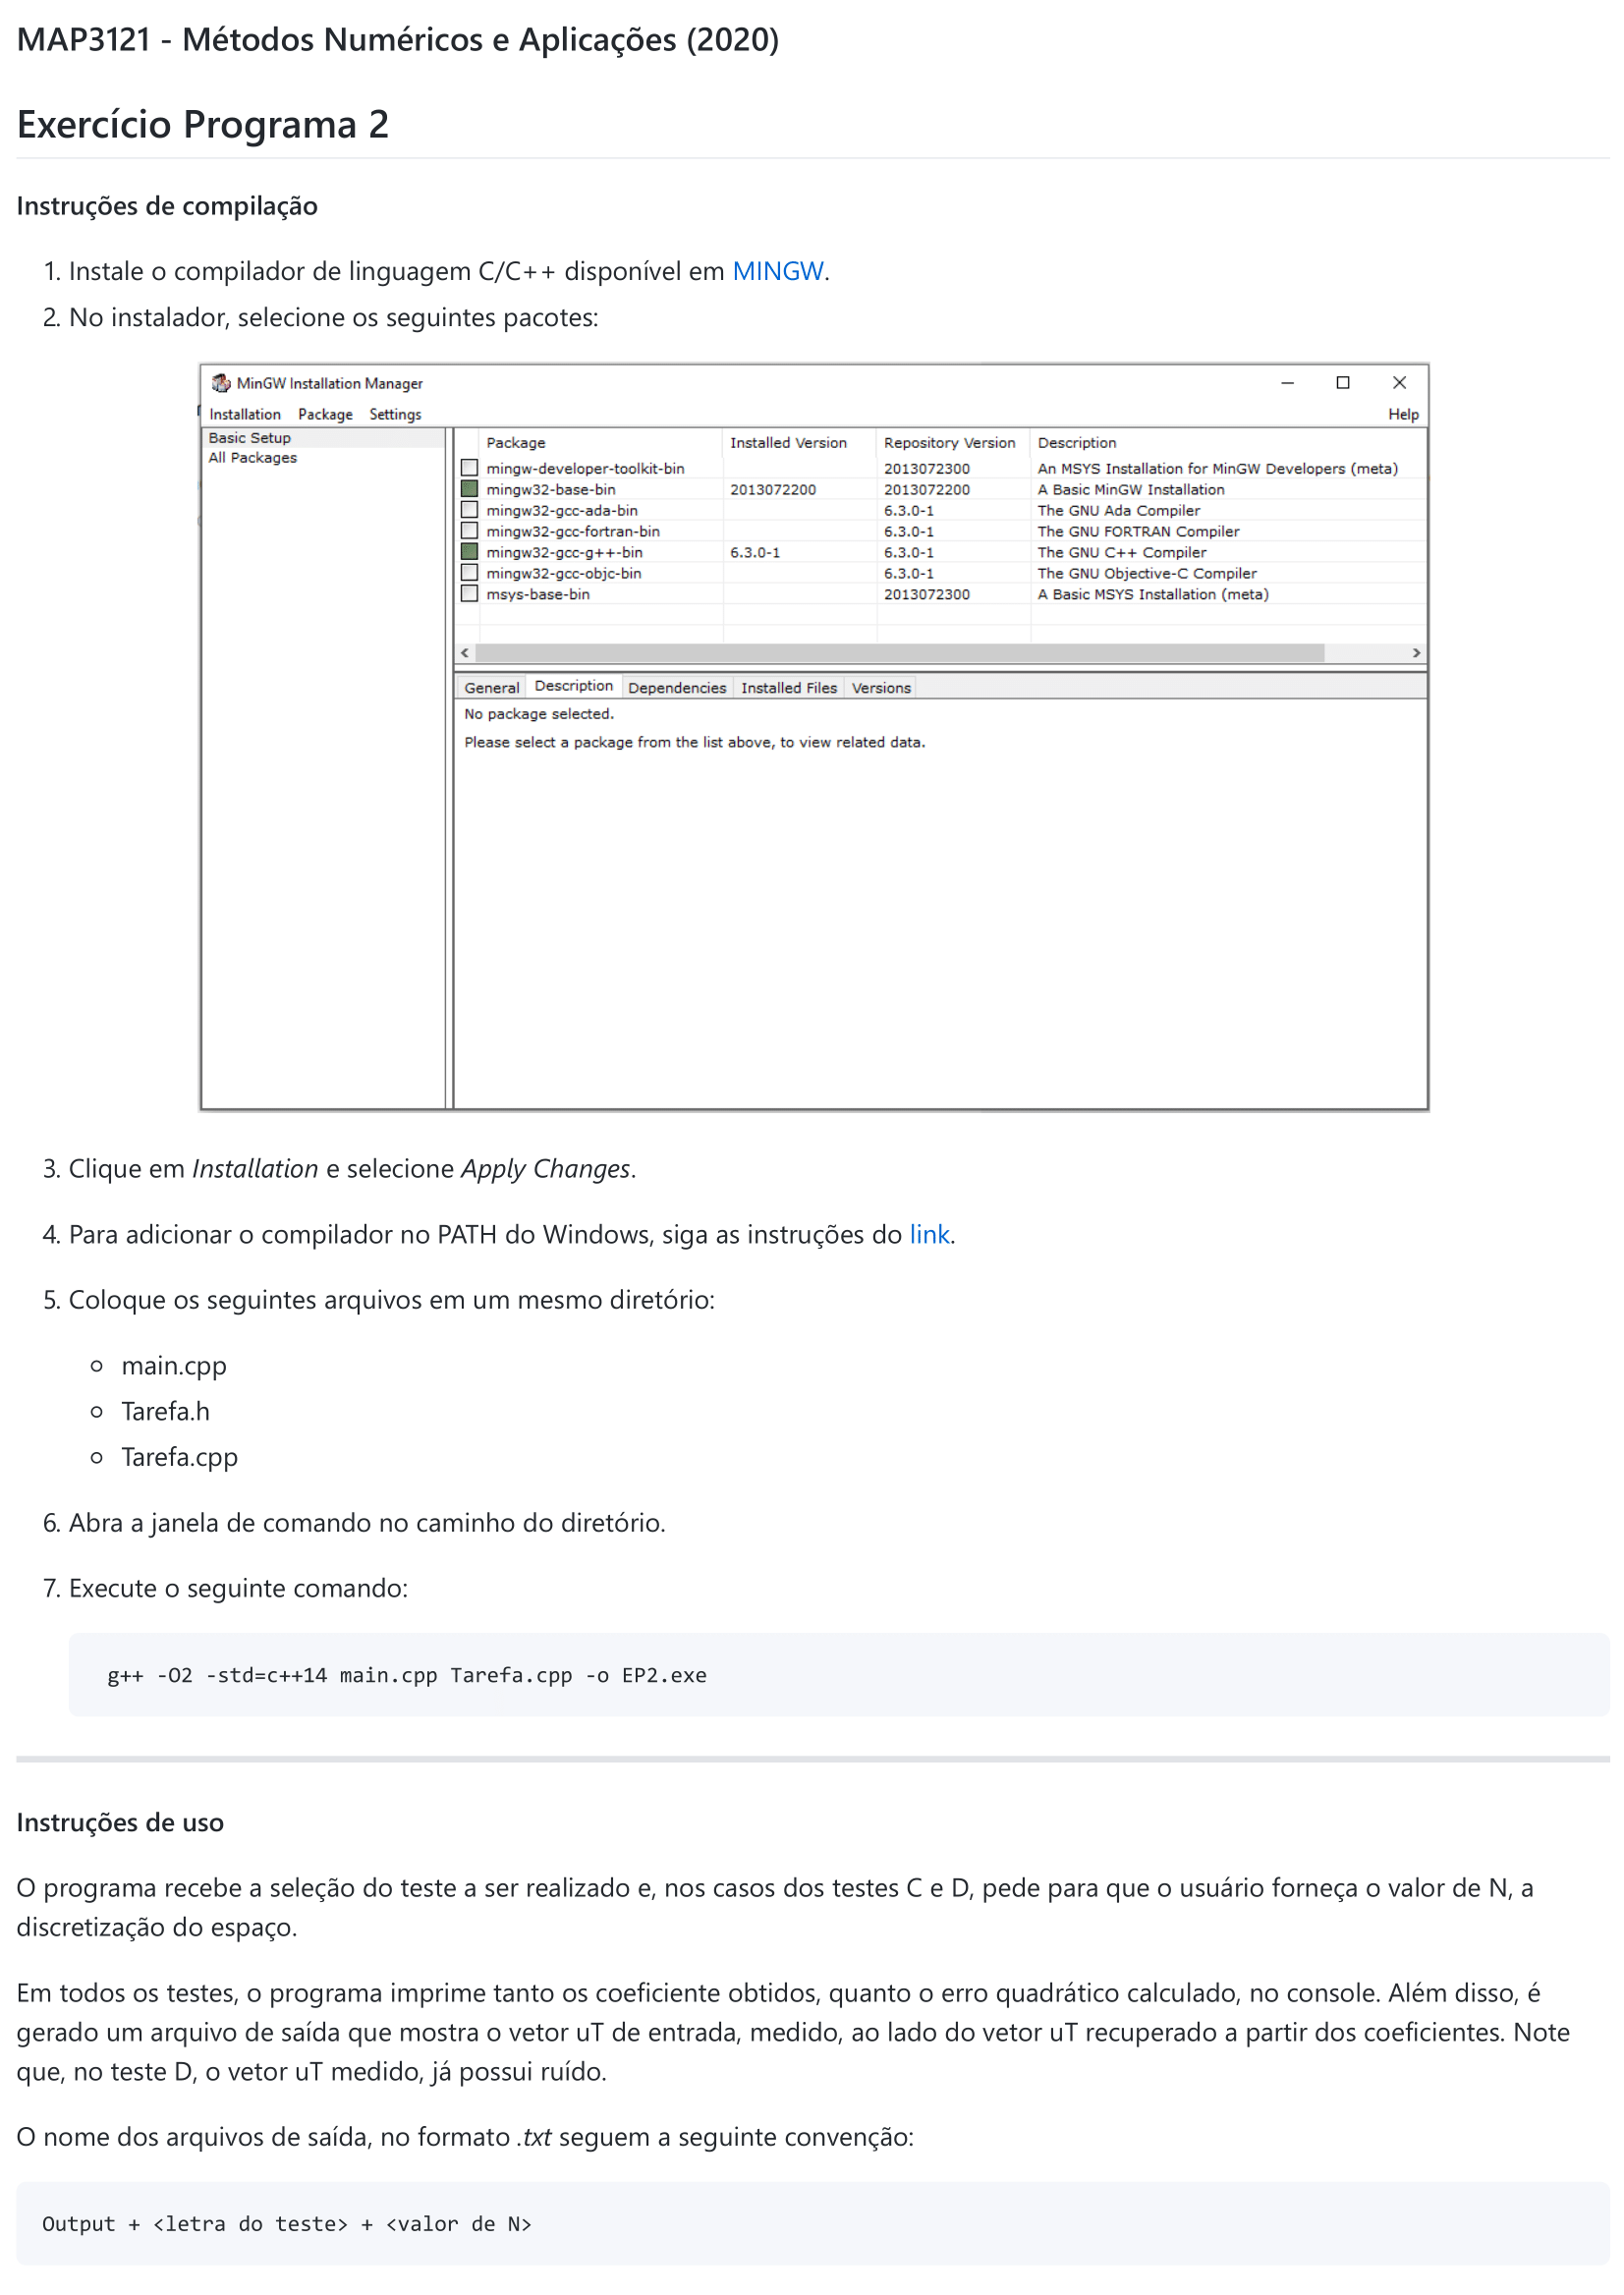
\includegraphics[width=0.9\linewidth]{README.png}
\end{figure}
\renewcommand{\footnotesize}{\tiny}
\footnotetext{\url{https://github.com/eliasrr1/EP2-Numerico}}

\end{spacing}
\end{document}
